\subsection{Creación de la empresa, vinculación del usuario e ingreso}
Con los endpoints creados, ya es posible realizar todas las acciones necesarias para integrar Mezfer Insider con CMS.

Lo primero que se tiene que hacer es crear la empresa, y para eso se llena un formulario con todos los datos de la empresa (Ver Figura 2).
    \begin{figure}[H]
        \begin{center}
            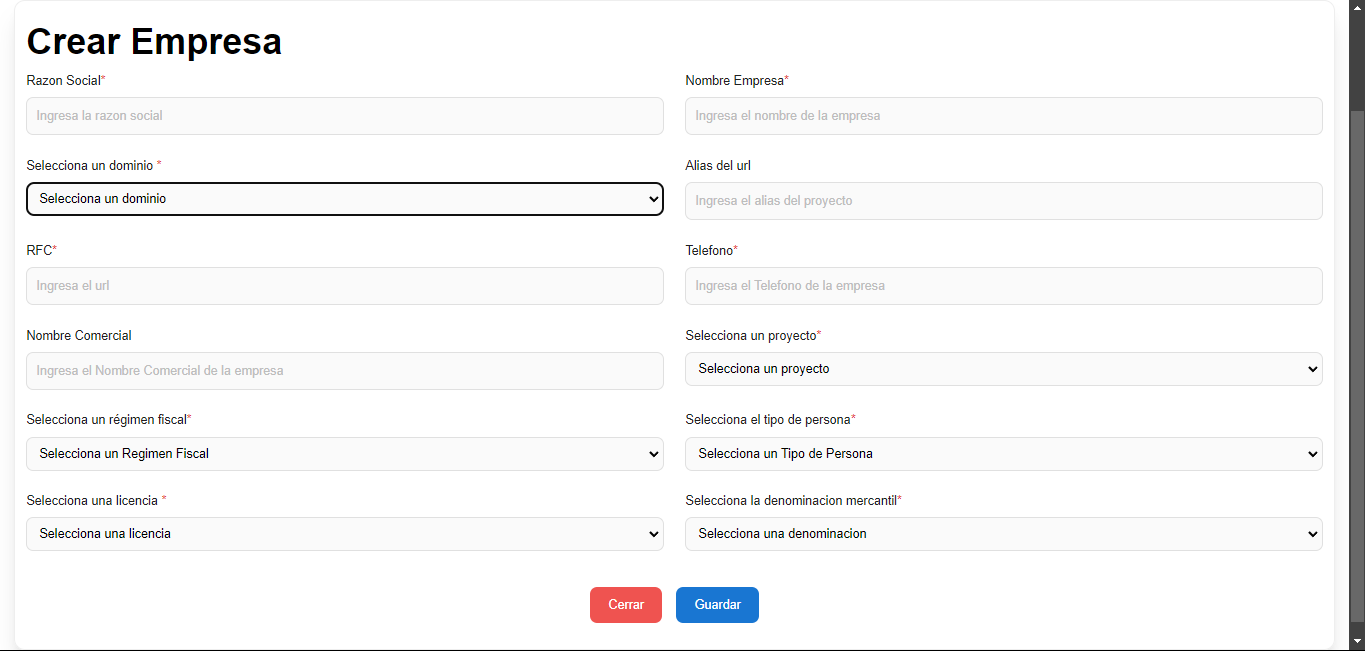
\includegraphics[scale=0.35]{img/actividades/integracion/formulario-empresa.png}
            \caption{Formulario para la creación de empresa.}
            \label{fig:formulario-empresa}
        \end{center}
    \end{figure}
Posteriormente, el usuario debe ser vinculado con la empresa (Ver Figura 3).
    \begin{figure}[H]
        \begin{center}
            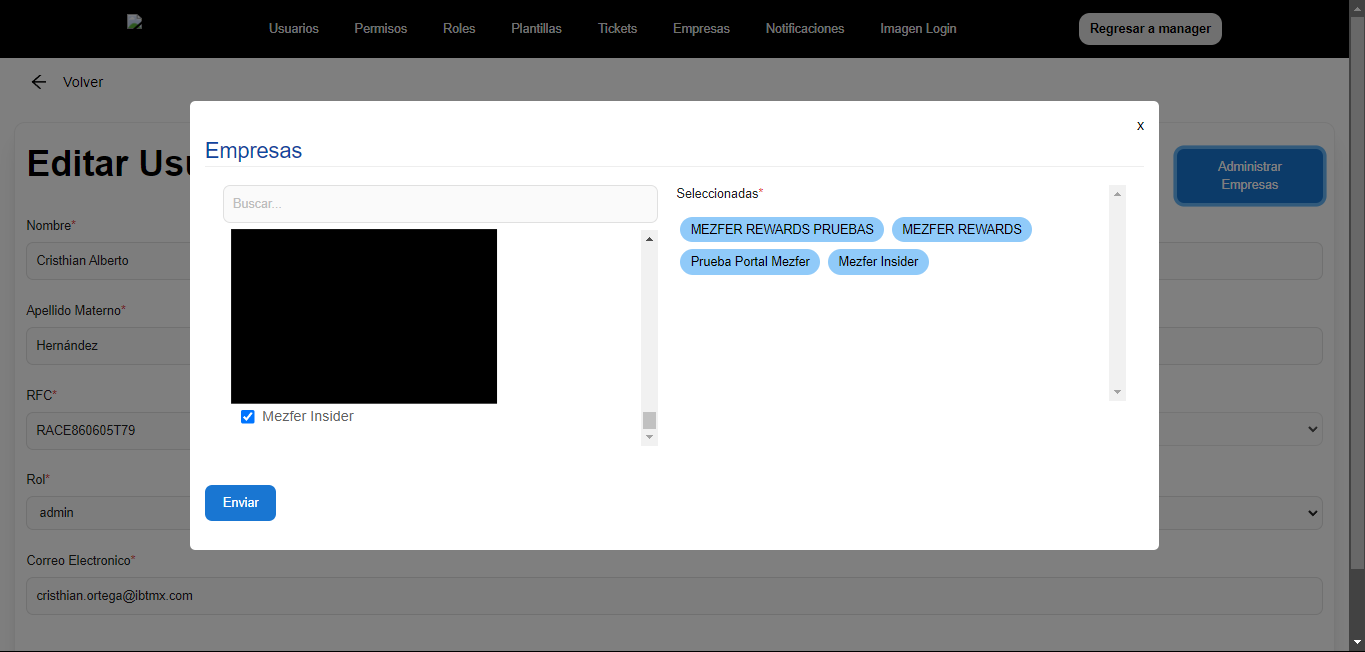
\includegraphics[scale=0.35]{img/actividades/integracion/vincular-usuario.png}
            \caption{Vinculación de usuario con empresa.}
            \label{fig:vincular-usuario}
        \end{center}
    \end{figure}
Y con esto realizado, el usuario ya podrá tener acceso a la empresa (Ver Figura 4).
    \begin{figure}[H]
        \begin{center}
            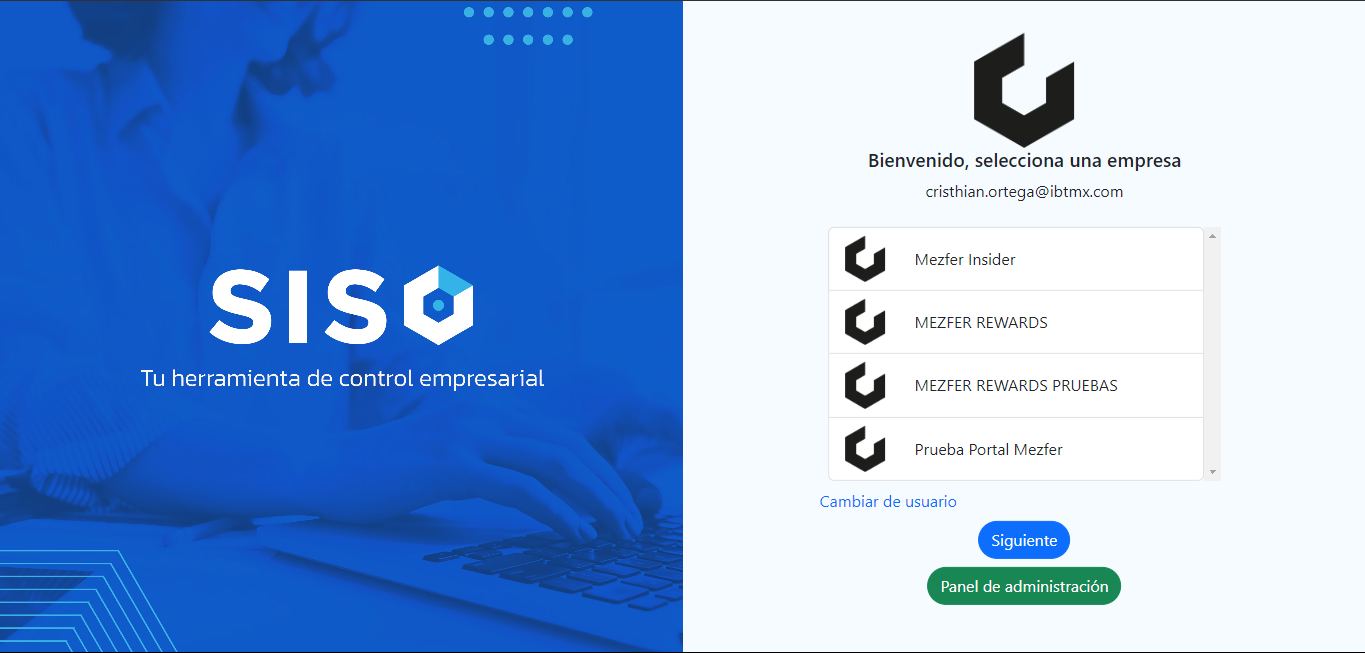
\includegraphics[scale=0.35]{img/actividades/integracion/ingreso-empresa.png}
            \caption{Selección de empresa.}
            \label{fig:ingreso-empresa}
        \end{center}
    \end{figure}